\section{项目的主要内容和技术路线}
\par 本研究的主要内容主要是在宫颈细胞学的图像上实现宫颈病变细胞的检测,主要关注检测过程中单细胞和细胞簇检测的任务分解和基于半监督学习的利用正常细胞特征辅助病变细胞检测方法。

\subsection{主要研究内容}
\subsubsection{任务分解}
\par 在自然图像的目标检测过程中每个类别都有固定的含义,每一个标注框都明确地指明一个完整的物体。例如,在行人检测的任务中,每一个检测框都会对应一个完整的行人,即使是多个行人挨在一起,也不会用一个标注框同时框住多个行人。但是,在TCT图像中这一点并不成立,有时会有大量的病变细胞聚集在一起形成一个大型的细胞簇,医生在标注的过程中很难准确地区分出每个细胞,同时逐一标注出每个病变细胞又太过耗时费力,而在实际使用模型的时候,我们是可以接受一个框住整个细胞簇的框的。因此,TCT的图像中同一类别的框既可能代表着单个的该类别的病变细胞,也可能代表着一整个该类别病变细胞形成的细胞簇,这就带来了很大的语义差异。
\begin{figure}[h]
    \centering
    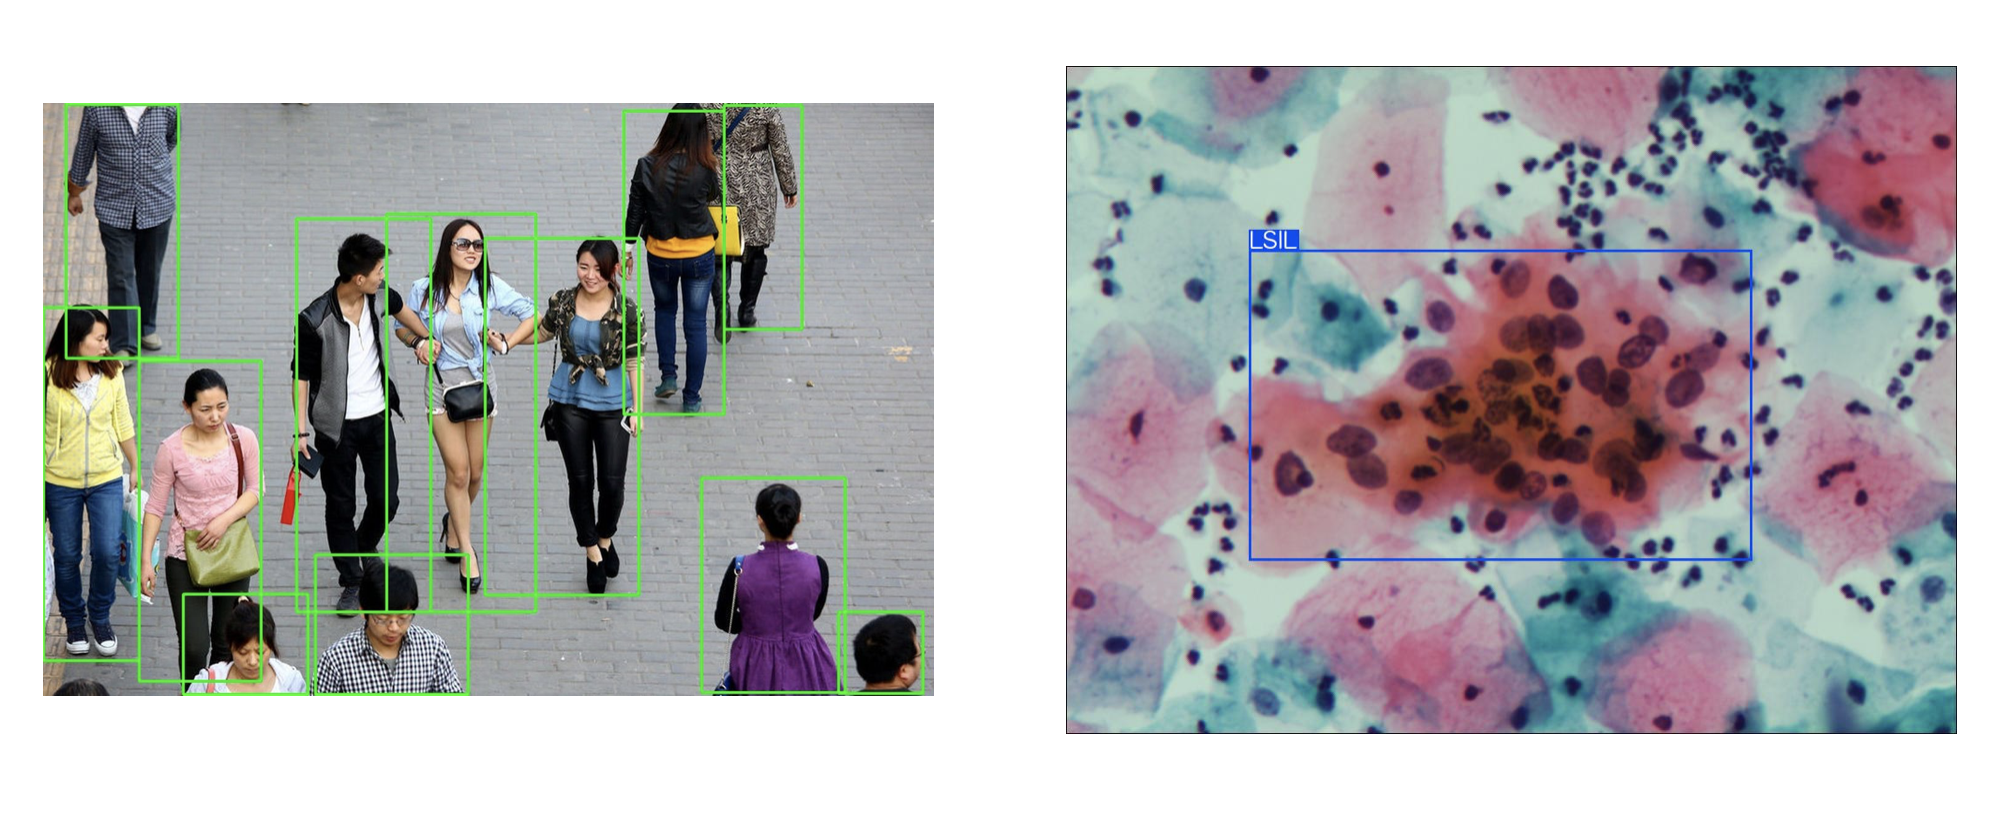
\includegraphics[width=0.5\paperwidth]{TCT/行人与TCT.png}
    \caption{在行人检测中每个行人都会对应一个检测框。而TCT图像中,有时会很难区分出单个的病变细胞,同时为每个病变细胞标注检测框又会带来不必要的高昂成本}
    \label{行人与TCT}
\end{figure}
\par 此外,如\ref{单细胞多细胞形态差异}所示,细胞簇还会具有着与单个细胞完全不同的形态特征。单个细胞往往成近似圆形或椭圆形,一般细胞的中心是细胞核周围是细胞质;而细胞簇的形状完全取决于混匀过程中各个细胞粘合在一起时的形态,并不固定,细胞簇中心的特征与边缘的特征是某些处于细胞簇中心或边缘的细胞的特征而非相应的细胞组分(细胞核、细胞质)的特征,因此,细胞簇中心的特征和边缘的特征在形态上都不会有特别明显的区别。这就带来了很大的形态特征差异。
\begin{figure}[h]
    \centering
    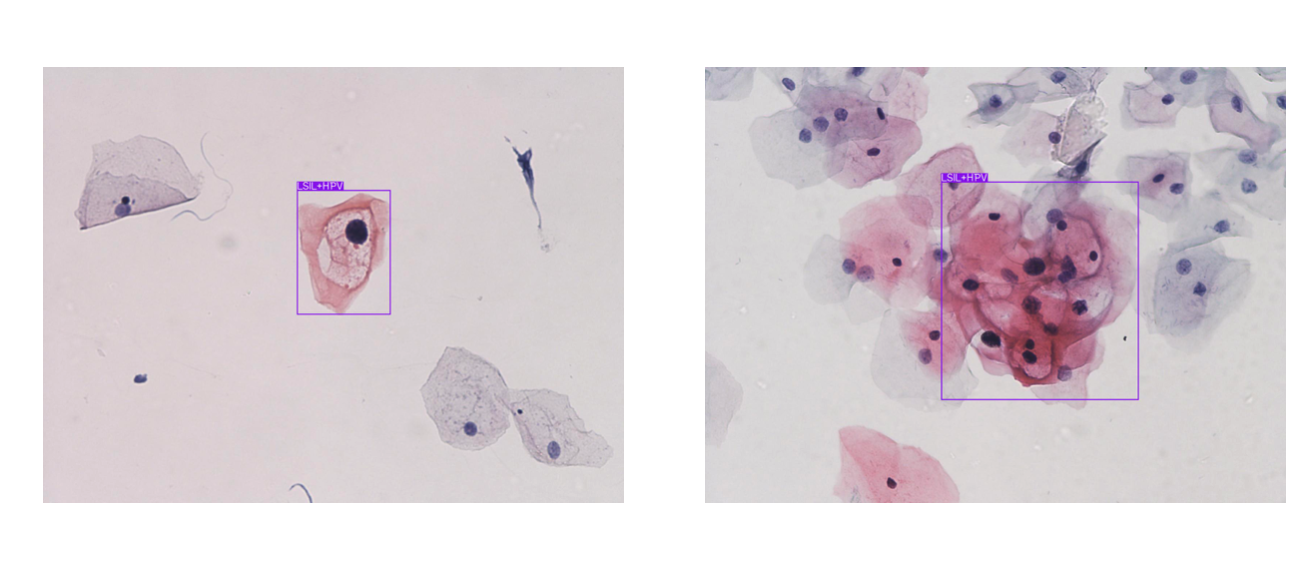
\includegraphics[width=0.5\paperwidth]{TCT/single_multi.png}
    \caption{单个病变细胞与病变细胞簇形态差异比较,左图为单个病变细胞,右图为许多病变细胞形成的细胞簇,两图中的病变细胞均为统一病变等级,但是由于细胞数目不同而具有完全不同的形态特征}
    \label{单细胞多细胞形态差异}
\end{figure}
\par 由此,如果我们使用同样的标注注明这两类不同的细胞、用同一个网络去学习检测这两类细胞,那么,网络在学习的过程中很可能遇到特征之间的冲突,因而无法很好地捕捉到这两类病变细胞所公有的特征。因此,我们希望将病变细胞检测这个整体任务分解为分别预测单个该种类病变细胞与预测该种类病变细胞簇两类任务,并通过使用不同的网络分别完成这两类任务,这样不同的网络专门负责某一类的细胞,网络就可以在学习的过程中避免语义特征和形态特征上的冲突,从而更好地捕捉这两类病变细胞的特征,进而促进模型的学习过程、提高模型的检测精度。
\subsubsection{半监督学习}
\par TCT检查的结果图片都是经由显微镜放大之后获得的,因此,图片上的细胞或细胞成分的绝对大小只取决于所使用的放大倍数而与实际情况无关,只有同一图像上各个细胞或细胞成分的相对大小才是有意义的。如\ref{放大倍率差异}所示,不同图片之间有着较大的放大倍率差异,因此,只能根据同一图片中正常细胞的大小作为判断的基准。在临床上,医生在做TCT诊断时,也是根据图像中正常细胞的细胞核、细胞质等组分的大小作为依据,通过对比病变细胞的相应细胞组分与正常细胞相应细胞组分的大小比例来判断病变细胞的等级的。由此,我们希望模型在检测病变细胞之外,也提取出部分正常细胞的形态、尺寸等特征用于辅助病变细胞的检测过程。
\begin{figure}[h]
    \centering
    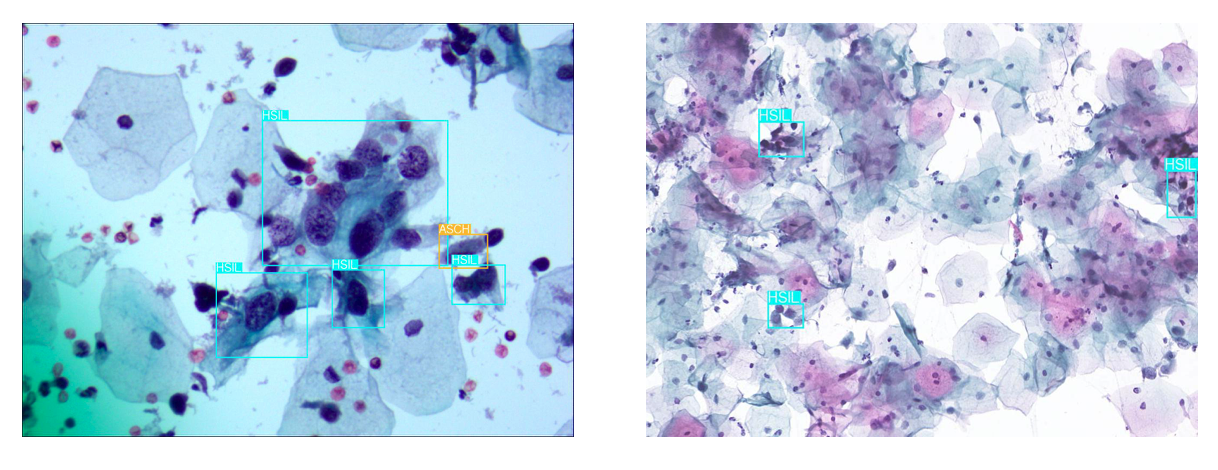
\includegraphics[width=0.5\paperwidth]{TCT/scale.png}
    \caption{不同图片之间放大倍率有着较大的差距,左图中的正常细胞大小相较右图中大得多,而实际上正常细胞的大小应当是一致的,所以左图放大倍率应当比右图高很多}
    \label{放大倍率差异}
\end{figure}
\par 但是,由于大多数TCT图像的病变程度不是很高,图像中正常细胞的数目会远远多于病变细胞。因此,在实际操作过程中,我们不可能要求医生在诊断的过程中除了标注出病变细胞以外还指明涂片中的所有正常细胞。由此,我们希望通过一些半监督的方法,如知识蒸馏等,让模型利用一部分带有标注的正常细胞和大量的未标注的正常细胞的形态等特征信息学习到检测正常细胞的方法,并能够提取出正常细胞的形态,细胞核、细胞质等组分的尺寸等特征,用于促进病变细胞的检测。
\subsection{技术路线}
\par 如\ref{模型结构}所示,我们的模型依然遵循上述问题主要分为任务分解和半监督学习两个部分。模型会先使用一个卷积神经网络和相应的FPN模块提取图像的特征。之后特征会被用于分别检测正常细胞,这一部分的检测会用到知识蒸馏等半监督学习方法。随后,CNN提取出的图像特征和正常细胞检测模型中提取出的正常细胞的特征会被综合在一起用于异常细胞的检测,这一部分将会使用任务分解的思想。这一部分的输出就是整个模型的最终预测结果。
\begin{figure}[h]
    \centering
    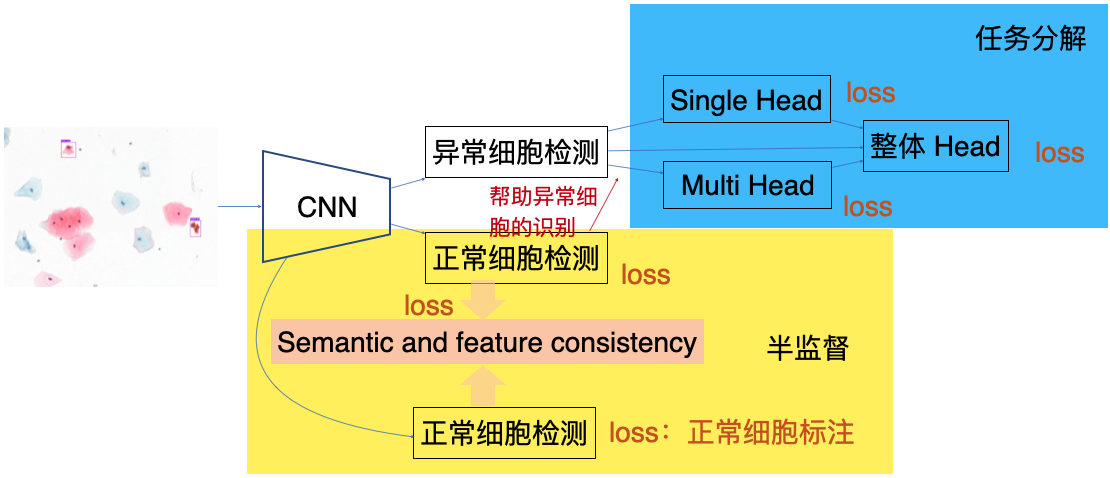
\includegraphics[width=0.7\paperwidth]{TCT/Network.png}
    \caption{模型大致的结构}
    \label{模型结构}
\end{figure}
\subsubsection{任务分解}
\par 任务分解的想法主要用在异常细胞识别的过程中。如前文所述,单个细胞和多个细胞组成的细胞簇有着较大的形态上和语义上的差异,如果将它们混在一起由网络学习,势必会导致特征上的冲突,阻碍网络捕捉病变相关的特征信息。因此,我们为单个细胞和细胞簇这两类不同的任务设计了两个不同的head,他们只会与相对应的标注数据计算损失。例如,single head在计算损失时,只考虑单个细胞所对应的标注框而忽略细胞簇的标注框;multi head则恰恰相反,它只考虑细胞簇的标注框而忽略单个细胞的标注框。这样的设计让两个不同的head捕捉不同的目标会更有利于网络捕捉到目标的形态特征,可以促进网络的学习过程。这之后,single head和multi head的预测结果以及他们提取出的不同的区域的图像特征都会在最终阶段被整体head所接受以做出最后的预测结果。这样的设计既让网络可以更好得捕捉不同目标的不同形态特征,又可以综合分类各种类别的特征以评定病变等级,可以进一步提升模型的预测精度。
\par 除此之外,在异常细胞检测过程中的三个head都还会接受来自正常细胞检测过程的结果和代表着正常细胞的形态、尺度等特征,这也会帮助异常细胞检测的模型更好得判断病变等级。
\subsubsection{半监督学习}
\par 在正常细胞的检测过程中,由于我们希望尽可能少地使用正常细胞的标注数据,并模拟实际使用中没有全部标注正常细胞的情况,我们只额外标注出少部分的正常细胞提供给模型学习,但数据集中含有大量的未被标注的正常细胞。因此,我们需要使用知识蒸馏等半监督学习的方法来利用这些无标注的正常细胞数据,以达到模型可以顺利捕捉正常细胞形态、尺寸等特征信息的目的。由此,我们在这个阶段设计了两个同样的head,一个用作教师head,一个用作学生head。教师head可以正常地获得数据集中正常细胞的标注,并通过计算损失函数、反向传播梯度等方法正常地进行优化学习;而学生head只会获得教师head预测的标签,并将自己的预测结果与教师head预测的结果输入到损失函数中计算损失。除此之外,学生head和教师head每层的特征还会通过一个一致性损失来保证一致性。通过这种方式,学生head就可以模拟教师head的预测过程学习到如何检测正常细胞。这样模型就可以利用数据集中没有标注的正常细胞的信息,以更好地捕捉正常细胞的形态特征,并最终促进网络的学习。

\subsection{可行性分析}
\subsubsection{任务分解}
\par 目前已有许多研究使用任务分解的方法来促进模型捕捉相应目标的形态特征。以Yu等\cite{zhang2019decompose}为例,该文章是在医学图像上做多类别的分割任务,如\ref{任务分解}所示,作者将同一个类别的目标根据目标形状的不同人为地划分为不同的类别,然后对每个类别分别使用一个模块进行分割,并在最后使用一个统一的模块进行综合处理。该做法确实地提高了模型捕捉不同目标形态特征的能力,相较于其选用的基准模型,该方法在不同数据集上检测效果均有部分提升。由此,任务分解的方法应当是可行的。
\begin{figure}[h]
    \centering
    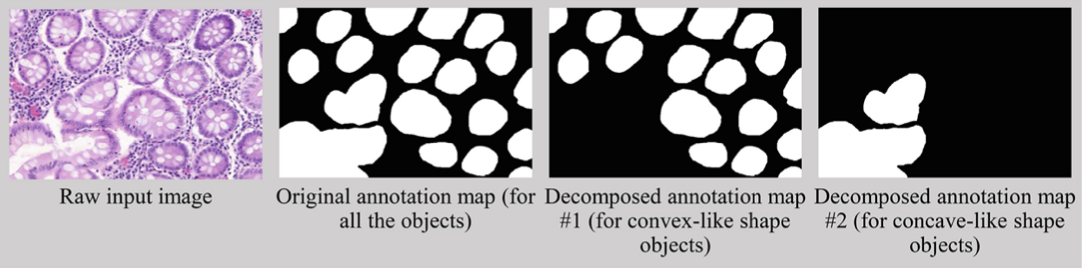
\includegraphics[width=0.5\paperwidth]{TCT/任务分解.png}
    \caption{根据目标的形状将同一个类别的目标人为地划分成多个类别}
    \label{任务分解}
\end{figure}
\subsubsection{基于正常细胞的对比}
\par 在临床诊断的过程中,医生也是根据图像中正常细胞的细胞核、细胞质等细胞成分的大小作为基准,根据病变细胞相应成分的大小、形态等特征的变化来判断病变细胞等级的。由此,基于正常细胞的特征通过比较的方法检测和判定病变细胞及其等级应当是可行的。
\par 此外,如\ref{比较检测}所示,Liang等\cite{liang2018comparison}通过一些从数据集中提取出来的参考样本生成每个类别的原型表示,并通过这种原型表示与CNN从输入图片提取出来的特征进行对比完成最终的分类任务。这种方法相较于基准模型,获得了不错的性能提升。由此,这种方法在我们的数据集上应当也是可行的。
\begin{figure}[h]
    \centering
    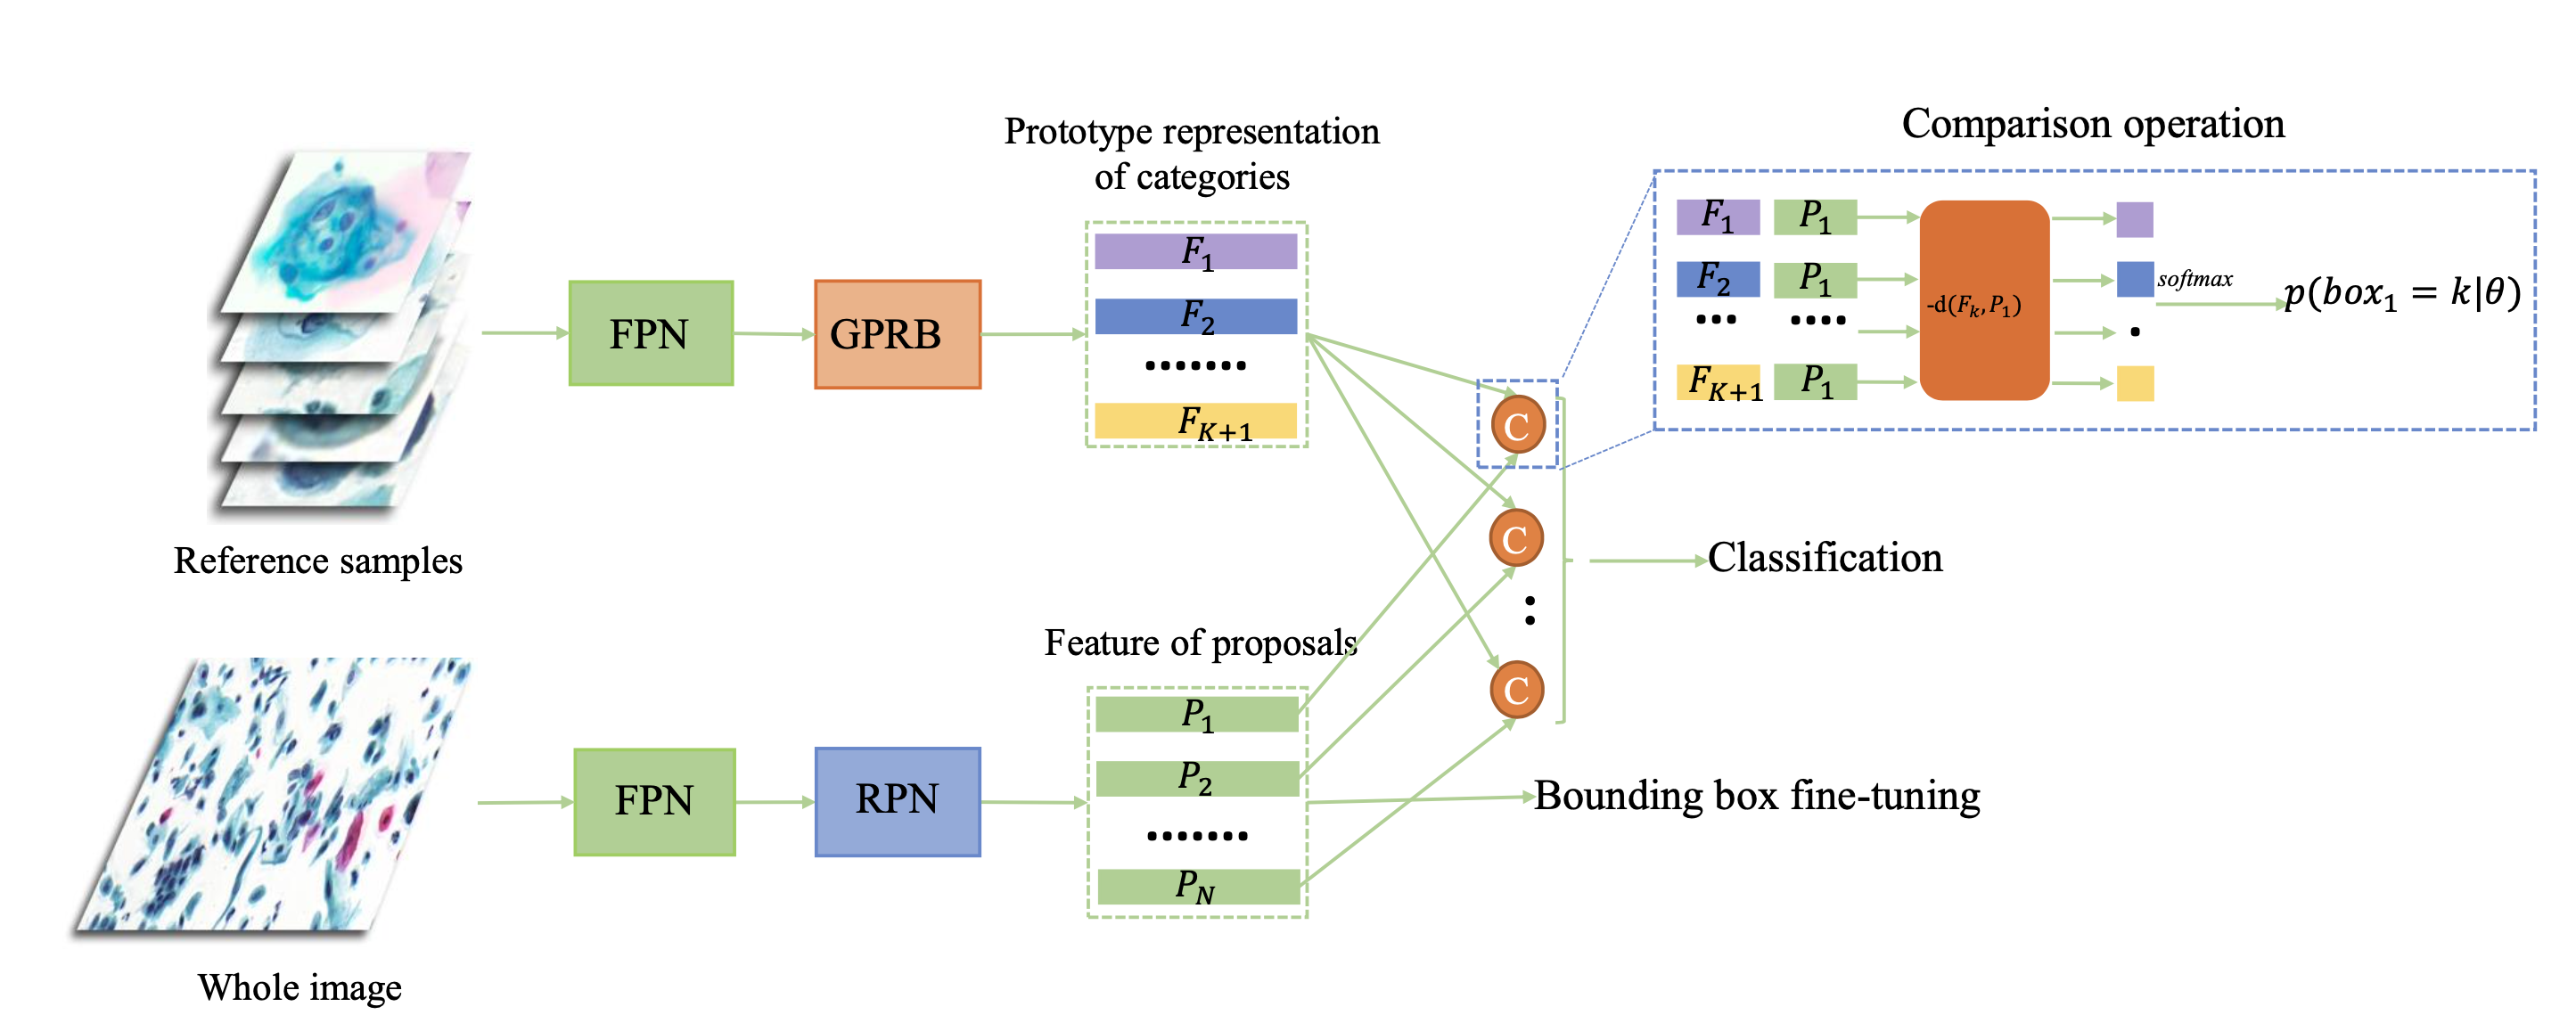
\includegraphics[width=0.5\paperwidth]{TCT/比较检测.png}
    \caption{比较检测器的网络结构}
    \label{比较检测}
\end{figure}
\subsubsection{半监督}
\par 由于医学数据集的标注通常需要专业的医师来完成,大量的标注数据往往代表着高昂的成本,因此,在医学相关的深度学习领域已经有许多研究通过半监督的方法让模型可以利用到大量的无标注的数据,并以此来提升模型捕捉目标形态特征的能力。
\par Lequan Yu等\cite{yu2019uncertainty}就通过知识蒸馏等半监督学习方法让模型可以利用更多的无标注信息,并以此提高了模型捕捉目标形态特征的能力,最后提高了模型分割结果的准确度。
\begin{figure}[h]
    \centering
    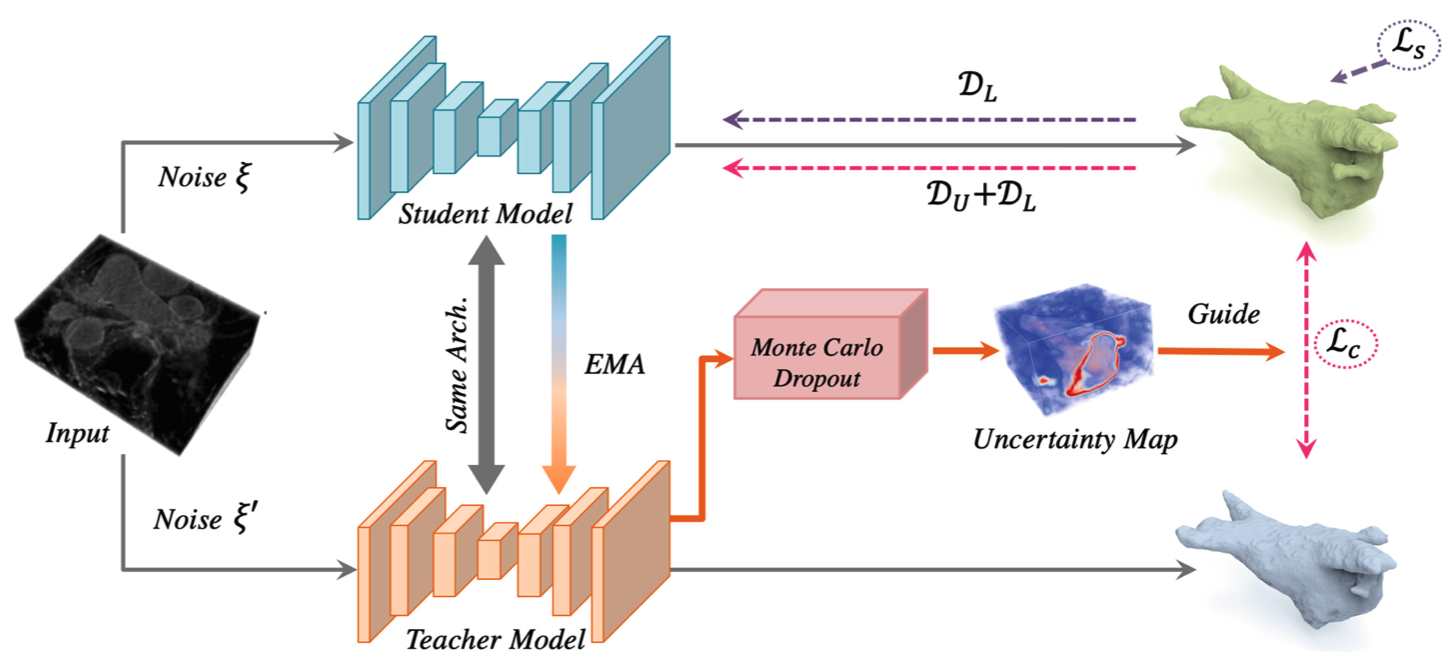
\includegraphics[width=0.5\paperwidth]{TCT/半监督.png}
    \caption{使用知识蒸馏等半监督学习方法的分割网络结构}
    \label{半监督}
\end{figure}
